\section{Webové aplikace}

Webová aplikace je typ počítačového software, který je uživateli sdílen prostřednictvím internetu. 
Uživatel se k~aplikaci dostane pomocí webového prohlížeče a~nemusí si ji instalovat na svůj počítač. 
Aplikace jsou jakýmsi prostředníkem mezi uživatelem a~serverem, kde se nachází data a~logika aplikace.\cite{codeacademywebapp}

Předpokládáme, že čtenář má základní znalosti HTML, CSS a~JavaScriptu. 
Tato znalost usnadní proces a~pomůže čtenáři lépe porozumět konceptům a~technikám, které zde budou popsány.

\subsubsection*{Frontend a Backend}

Uživatelské rozhraní, se kterým uživatel přímo interaguje, nazýváme frontend, neboli klient.
Úkolem klienta je zobrazovat vizuální stránku uživateli a~zpracovávat jeho vstupy. 
Mezi klíčové frontendové technologie patří HTML, CSS a~JavaScript.

Backend, či také server, je část aplikace starající se o~zpracování dat a~logiku aplikace. 
Backend se skládá z~databází a~algoritmů, komunikuje s~klientem prostřednictvím API a~zpracovává požadavky. 
Serverovou část lze implementovat v~široké škále programovacích jazyků, např.~v~Pythonu, Javě, PHP, Ruby, JavaScriptu.\cite{stateofartframeworks}

\begin{figure}[htb]
	\centering
		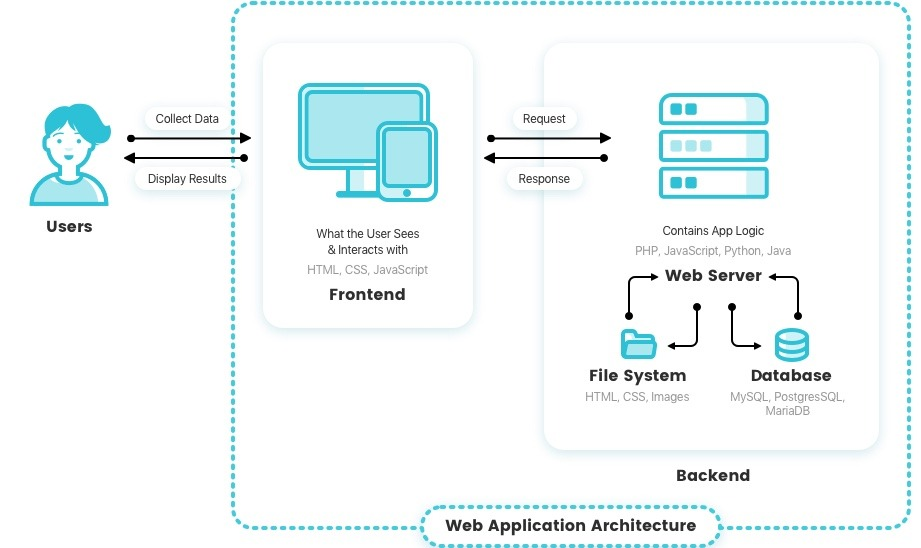
\includegraphics[width=1\textwidth]{images/webapparchitecture.jpg}
	\caption[Diagram architektury webových aplikací]{Diagram architektury webových aplikací \cite{webappsarchitecture}}
	\label{fig:webappsarchitecture}
\end{figure}

\subsubsection*{Single Page Application}

Pod pojmem Single Page Application (SPA) rozumíme webové aplikace, které se skládají z~jediné stránky a~také jednotlivých částí aplikace. 
Obsah stránek bývá dynamicky aktualizován pomocí JavaScriptu. Tento přístup umožňuje aktualizaci stránek bez nutnosti obnovování celé stránky. 
V~praxi to znamená, že při jakékoli akci uživatele se aktualizuje pouze obsah stránky, nikoli celá stránka. 
Mezi výhody tohoto přístupu patří rychlejší odezva aplikace, méně dotazů na server a~také lepší uživatelský zážitek.\cite{jadhavspa}

\begin{figure}[htb]
	\centering
		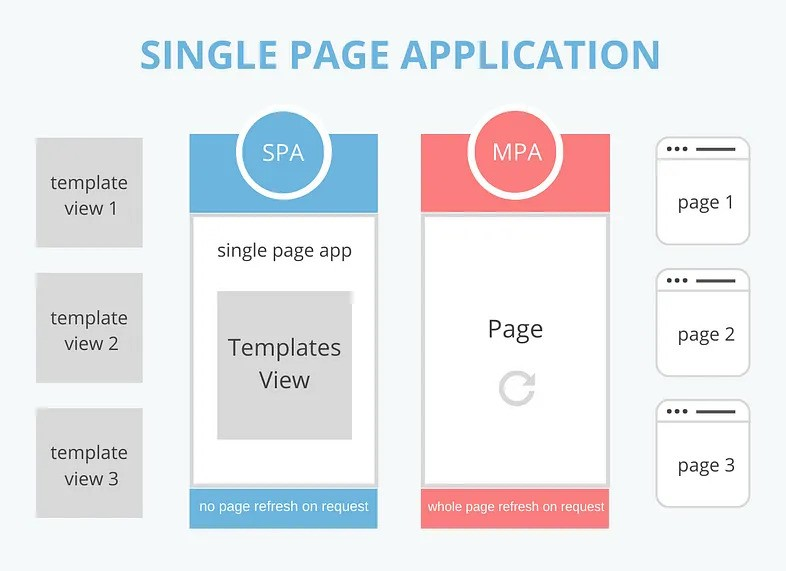
\includegraphics[width=.75\textwidth]{images/SPAvsMPA.jpg}
	\caption[Single Page Application oproti klasické webové stránce (Multi Page Application)]{Single Page Application oproti klasické webové stránce (Multi Page Application) \cite{fergusonspavsmpa}}
	\label{fig:spavsmpa}
\end{figure}

\subsubsection*{Framework}

Framework je software, který poskytuje architekturu a~nástroje pro rychlejší a~jednodušší vývoj daných aplikací. 
Vývojář při využití frameworku nemusí řešit základní problémy, které jsou již vyřešeny v~samotném frameworku. 
Použití frameworku snižuje technický dluh, zlepšuje rozšiřitelnost a~flexibilitu aplikace. 
Zlepšuje také přenositelnost, spolehlivost a~škálovatelnost aplikace.\cite{schmidtframeworks}